\documentclass[10pt, a4paper]{article}


%%%%%%%%%%%%%%%%%%%%%%%%%%%%%%%%%%%%%%%%%%%%%
%%% Margens do documento.
%%%%%%%%%%%%%%%%%%%%%%%%%%%%%%%%%%%%%%%%%%%%%
\usepackage{anysize}                    % Pacote para configurar as margens do documento.
\usepackage[margin = 2.0cm, left = 3.0cm, right = 3.0cm, top = 2.0cm, bottom = 2.0cm, headheight = 16pt]{geometry}


%%%%%%%%%%%%%%%%%%%%%%%%%%%%%%%%%%%%%%%%%%%%%
%%% [CONFIGURACAO]:   TABELAS e GRAFICOS.
%%%%%%%%%%%%%%%%%%%%%%%%%%%%%%%%%%%%%%%%%%%%%
\usepackage[pdftex]{graphicx, color}    % Pacote de configuracao grafica.
\usepackage[table, xcdraw]{xcolor}      % Pacote de cores.
\usepackage[hidelinks]{hyperref}        % Pacote para configurar os links das referencias.
\usepackage{tabularx, multirow}         % Pacote para configuracao de tabelas.
\usepackage{booktabs}                   % Pacote para melhorar a qualidade das tabelas.
\usepackage{subfig}                     % Pacote para configurar subfiguras.
\usepackage{float}                      % Pacote para definir objetos inteiros (Como figuras e tabelas) como float.
\usepackage{array}
\usepackage{adjustbox}


%%%%%%%%%%%%%%%%%%%%%%%%%%%%%%%%%%%%%%%%%%%%%
%%% [CONFIGURACAO]: FONTES e TEXTOS.
%%%%%%%%%%%%%%%%%%%%%%%%%%%%%%%%%%%%%%%%%%%%%
\usepackage[utf8]{inputenc}             % Pacote para configurar o padrao de caracteres.
\usepackage[portuges, brazilian]{babel} % Pacote para configuracao de linguagem.
\usepackage{amssymb, amsmath}           % Pacote com padroes de linguagem e texto matematico.
\usepackage{enumerate}                  % Pacote para configuracao das listas enumeradas.
\usepackage{caption}                    % Pacote para configurar os captions.
\usepackage{natbib}                     % Pacote para configurar as citacoes.
\usepackage{ifthen}                     % Pacote para criar comandos condicionais.
\usepackage{parskip}                    % http://ctan.org/pkg/parskip
\usepackage{titlesec}                   % Pacote para formatar os titulos.

\titleformat{\section}{\normalfont\fontsize{12}{15}\bfseries}{\thesection}{1em}{}[{\titlerule[1pt]}]    % Configuracao dos titulos.
\setlength{\parindent}{0pt}
\renewcommand{\baselinestretch}{1.5}
\allowdisplaybreaks                     % Permite a quebra de página entre equacoes.


%%%%%%%%%%%%%%%%%%%%%%%%%%%%%%%%%%%%%%%%%%%%%
%%% [CONFIGURACAO]: CABECALHOS e RODAPES.
%%%%%%%%%%%%%%%%%%%%%%%%%%%%%%%%%%%%%%%%%%%%%
\usepackage{fancyhdr}           % Pacote para configuracao de cabecalhos e rodapes.
\usepackage{afterpage}
\pagestyle{fancy}               % Define um estilo de pagina com cabecalho.
\fancyhf{}                      % Remove as configuracoes de cabecalho e rodape.
\fancyhead[R]{                  % Define o cabecalho.
    \footnotesize
    Universidade Federal do Espírito Santo          \\
    Programa Institucional de Iniciação Científica  \\
    Relatório Final de Pesquisa                     \\
    Ciências Exatas e da Terra                      \\
}
\renewcommand{\headrulewidth}{0pt}  % Tamanho da linha horizontal abaixo do cabecalho.
\fancyfoot[R]{\thepage}             % Define o rodape.

\pagenumbering{arabic}
\usepackage{verbatim}   % Pacote para comentar trechos do texto.
\usepackage{ragged2e}



% \newcommand{\Cor}{\cellcolor[HTML]{e6e6e6}}
\newcommand{\Cor}{\cellcolor[HTML]{E5E5E5}}



%%%%%%%%%%%%%%%%%%%%%%%%%%%%%%%%%%%%%%%%%%%%%
%%% [DOCUMENTO]:    INICIO.
%%%%%%%%%%%%%%%%%%%%%%%%%%%%%%%%%%%%%%%%%%%%%
\begin{document}

    \afterpage{\rfoot{\thepage}}
    
    \vspace*{1pt}
    \begin{center}
        {\Large \bf Métodos Exatos para o Problema de Corte Bidimensional com Dimensões Abertas - Piic/UFES}
    \end{center}
    % \vspace{.5cm}
    
    %\noindent
    \begin{tabularx}{\textwidth}{|l|X|}
        \hline
        \Cor {\bf Edital:}                              &   \textbf{Edital Piic 2022/2023.}                                              \\ \hline
        \Cor {\bf Grande Área do Conhecimento (CNPq):}  &   Ciências Exatas e da Terra.                                                  \\ \hline
        \Cor {\bf Área do Conhecimento (CNPq):}         &   Ciência da Computação.                                                       \\ \hline
        \Cor {\bf Título do Projeto:}                   &   Métodos Computacionais em Otimização.                                        \\ \hline
        \Cor {\bf Título do Subprojeto:}                &   Métodos exatos para o problema de corte bidimensional com dimensões abertas. \\ \hline
        \Cor {\bf Professor Orientador:}                &   Oberlan Christo Romão.                                                       \\ \hline
        \Cor {\bf Estudante:}                           &   João Victor do Rozário Recla.                                                \\ \hline
    \end{tabularx}
    \vspace{.5cm}


    %TODO: Deixar o texto impessoal

    %%%%%%%%%%%%%%%%%%%%%%%%
    %%% [RESUMO] %%%
%%%%%%%%%%%%%%%%%%%%%%%%
\section*{Resumo}

    Neste trabalho de conclusão de curso são propostos métodos de resolução para o problema de corte e empacotamento bidimensional com dimensões abertas. O capítulo de introdução descreve a aplicação do problema nas indústrias e as formas de solucioná-lo. No primeiro capítulo também são apresentados a hipótese de pesquisa e os objetivos do projeto. No capítulo de embasamento teórico são apresentados, de forma mais abrangente, a descrição do problema, os métodos de resolução propostos por outros autores e uma introdução as heurísticas e meta-heurísticas. No capítulo de metodologia são descritos a modelagem do problema e os meios utilizados para o desenvolvimento do projeto. No capítulo de resultados é apresentado uma discussão em cima dos resultados obtidos com a aplicação dos métodos de resolução propostos durante o estudo do problema. E no capítulo de conclusões, por fim, é apresentado uma conclusão para o trabalho realizado contendo a resposta para a hipótese de pesquisa.
    
    {\bf Palavras-chave:} Métodos exatos. Otimização. Problema de corte e empacotamento bidimensional. Strip Packing Problem 2D. Retangular. Não-guilhotinado.
    %%%%%%%%%%%%%%%%%%%%%%%%%%%%
    %%% [INTRODUCAO] %%%
%%%%%%%%%%%%%%%%%%%%%%%%%%%%
\section{Introdução}
    
    Indústrias como a do vidro, do aço e da madeira, entre outras que trabalham com o corte ou a embalagem de materiais, estão constantemente buscando otimizar seus processos produtivos para se manterem competitivas no mercado atual, altamente desafiador e globalizado. Buscar maneiras de reduzir o desperdício de matéria-prima é uma estratégia crucial para essas empresas, visando minimizar os custos de produção e melhorar a eficiência operacional (\cite{Morabito1998}), (\cite{hopper2000two}), (\cite{Morabito2000}), (\cite{Cintra2007}), (\cite{Parreno2021}). Nesse contexto, o problema de corte e empacotamento bidimensional, conhecido como \emph{Strip Packing Problem} (\emph{SPP}) 2D, desempenha um papel fundamental.

    No \emph{SPP-2D}, o objetivo é encontrar a melhor forma de alocar um conjunto de itens em um objeto bidimensional, de modo a minimizar o desperdício de área (\cite{hopper2000two}). A proposta original do problema é determinar a altura mínima do objeto necessário para atender às demandas de corte ou empacotamento dos itens (\cite{Cherri2009}). Essa abordagem está diretamente relacionada aos desafios enfrentados pelas indústrias mencionadas anteriormente. Diversos métodos de resolução foram desenvolvidos para maximizar a utilização da área disponível no objeto, considerando características como a forma dos itens (regulares ou irregulares), a possibilidade de rotação dos itens e o tipo de corte do objeto (guilhotinado ou não-guilhotinado).

    Os métodos propostos para o \emph{SPP} apresentam abordagens diferentes para resolver o problema. Com isso, para poder dizer se um modelo é eficiente ou não, é necessário realizar uma bateria de testes com instâncias já conhecidas na literatura e analisar o desempenho do método, na busca pela melhor configuração dos itens no objeto, considerando o tempo necessário para encontrar uma solução e a diferença entre os resultados já encontrados para o problema.

    Uma abordagem que pode ser considerada para solucionar o problema, otimizando a área aproveitada do objeto, é a redução do perímetro ou a redução da área. Esses modelos, de dimensões abertas, buscam encontrar uma configuração dos itens que minimize o espaço sobressalente no objeto, diferente da abordagem original, que trabalha com a largura fixa e visa minimizar apenas a altura do objeto.

    %%%%%%%%%%%%%%%%%%%%%%%%%%%%%%%%%%%%%%%%%
    %%% Exemplo da rotacao comentada.
    %%% Inserir outro exemplo sem rotacao.
    %%%%%%%%%%%%%%%%%%%%%%%%%%%%%%%%%%%%%%%%%
    \begin{comment}
        Na Figura~\ref{Fig-Exemplos-sem-rotacao} é apresentado um exemplo de aplicação desses três métodos, desconsiderando a rotação dos itens, para uma instância pequena. Nesse exemplo, a dimensão dos itens impede que os modelos encontrem a melhor configuração para o problema. Cada método consegue obter o melhor resultado para sua abordagem: o modelo do perímetro apresenta a configuração com o menor perímetro possível e o modelo da área apresenta a configuração que proporciona a menor área possível para o objeto, porém as soluções encontradas ainda podem ser melhoradas.
    
        %%% [FIGURA][EXEMPLO MODELOS SEM ROTACAO] %%%%%%%%%%%%%%%%%%%%%%%%%%%%%
        \begin{figure}[htbp]
            \centering
            \subfloat[Minimizar altura]{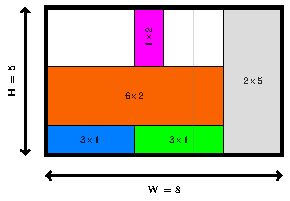
\includegraphics[scale = 1]{Figuras/Exemplo-modelo-altura.pdf}}
            \subfloat[Minimizar perímetro]{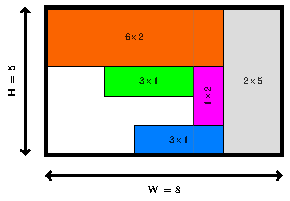
\includegraphics[scale = 1]{Figuras/Exemplo-modelo-perimetro.pdf}}
            \subfloat[Minimizar área]{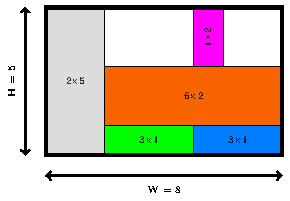
\includegraphics[scale = 1]{Figuras/Exemplo-modelo-area.pdf}}
            % \includegraphics{Figuras/nome.pdf}
            \caption{Exemplo de resolução do problema com três abordagens que desconsideram a rotação dos itens.}
            \label{Fig-Exemplos-sem-rotacao}
        \end{figure}
    
    
        Considerar a rotação dos itens em cada abordagem abre possibilidade para que novas configurações ótimas, que solucionem o problema, possam ser encontradas. Na Figura~\ref{Fig-Exemplos-com-rotacao} são exibidos o resultado dos mesmos modelos considerando a rotação dos itens. Nesse exemplo, os resultados mostram que ainda era possível otimizar a área aproveitada do objeto rotacionando alguns itens. Comparado ao primeiro exemplo, as soluções obtidas por esses métodos com a rotação dos itens demonstram ser ainda melhores: o modelo da altura conseguiu reduzir os espaços vagos e os modelos do perímetro e da área conseguiram entregar uma solução ótima com o máximo aproveitamento da área do objeto.
    
        %%% [FIGURA][EXEMPLO MODELOS COM ROTACAO] %%%%%%%%%%%%%%%%%%%%%%%%%%%%%
        \begin{figure}[htbp]
            \centering
            \subfloat[Minimizar altura]{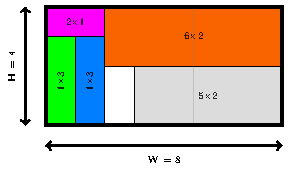
\includegraphics[scale = 1]{Figuras/Exemplo-modelo-altura-rotacao.pdf}}
            \subfloat[Minimizar perímetro]{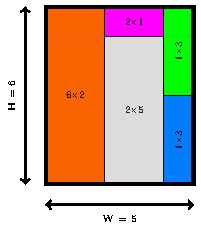
\includegraphics[scale = 1]{Figuras/Exemplo-modelo-perimetro-rotacao.pdf}} \\
            \subfloat[Minimizar área]{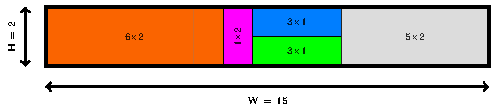
\includegraphics[scale = 1]{Figuras/Exemplo-modelo-area-rotacao.pdf}}
            % \includegraphics{Figuras/nome.pdf}
            \caption{Exemplo de resolução do problema com três abordagens que consideram a rotação dos itens.}
            \label{Fig-Exemplos-com-rotacao}
        \end{figure}
    \end{comment}

    Apesar da simplicidade, o problema de corte e empacotamento bidimensional é classificado como um problema \emph{NP-difícil} (\cite{Garey1990}), (\cite{Lodi2002}). Quanto maior a demanda de itens, mais tempo é necessário para o método aplicado encontrar uma solução. Sendo assim, %a utilização de heurísticas ou de meta-heurísticas, na resolução do problema, pode ser uma vantagem para encontrar melhores resultados no menor intervalo de tempo.
    é necessário buscar meios mais rápidos e eficientes para resolver o problema em menos tempo.

    Para otimizar o tempo de resolução do problema de corte e empacotamento bidimensional com corte não-guilhotinado, desconsiderando a rotação dos itens, é proposto neste projeto institucional de iniciação científica quatro métodos de solução, que consideram as dimensões do objeto (largura e altura) como abertas. Com isso, alguns testes serão realizados com instâncias presentes na literatura para analisar o desempenho do modelo exato formulado e comprovar se as abordagens apresentadas são realmente eficientes na resolução do problema.
    %%%%%%%%%%%%%%%%%%%%%%%%%%%
    %%% [OBJETIVOS] %%%
%%%%%%%%%%%%%%%%%%%%%%%%%%%
\section{Objetivos}

    %%%%%%%%%%%%%%%%%%%%%%%%%%%%%%%%%%
        %%% [OBJETIVOS GERAIS] %%%
    %%%%%%%%%%%%%%%%%%%%%%%%%%%%%%%%%%
    Os objetivos gerais desse projeto incluem a apresentação de quatro métodos de resolução para o \emph{SPP-2D} com dimensões abertas, considerando o problema de corte não-guilhotinado de um objeto retangular, sem a rotação ortogonal (Rotação de 90 graus) de itens retangulares, e a realização de uma análise de desempenho, a partir dos resultados obtidos com a resolução de várias instâncias do problema existentes na literatura, para identificar o método que encontra, no menor tempo de execução, a melhor configuração dos itens no objeto.
    
    
    %%%%%%%%%%%%%%%%%%%%%%%%%%%%%%%%%%%%%%%
        %%% [OBJETIVOS ESPECIFICOS] %%%
    %%%%%%%%%%%%%%%%%%%%%%%%%%%%%%%%%%%%%%%
    \newpage
    Os objetivos específicos da pesquisa são:
    
    \begin{itemize} %[align = parleft, left = 50pt..6em]
        \item Apresentar um modelo matemático para o problema, com quatro abordagens de resolução.
        \item Discutir o desempenho dos métodos desenvolvidos na resolução do problema.
        \item Apresentar os resultados do projeto respondendo à hipótese de pesquisa.
    \end{itemize}
    %%%%%%%%%%%%%%%%%%%%%%%%%%%%%%%%%%%%%
    %%% [EMBASAMENTO TEORICO] %%%
%%%%%%%%%%%%%%%%%%%%%%%%%%%%%%%%%%%%%
\section{Embasamento teórico}

    %%%%%%%%%%%%%%%%%%%%%%%%%%%%%%%%%%%%%%%%%%%%%%%%%%%
        %%% [PROBLEMA DE CORTE E EMPACOTAMENTO] %%%
    %%%%%%%%%%%%%%%%%%%%%%%%%%%%%%%%%%%%%%%%%%%%%%%%%%%
    \subsection{Problema de corte e empacotamento}
        
        O problema de corte ou empacotamento bidimensional também é classificado como um \emph{ODPP} (\emph{Open Dimensional Packing Problem}) (\cite{Wascher2007}), onde a largura $W$ do objeto possui um valor fixo e a altura $H$ do objeto é aberta, podendo assumir qualquer valor. Com isso, a resolução do problema \emph{SPP} consiste em encontrar a menor altura de $H$ que maximize o aproveitamento da área do objeto, permitindo a inserção de um conjunto de $N$ itens retangulares, sem sobreposição, com uma configuração ótima para o corte ou o empacotamento dos mesmos.

        Na literatura existem inúmeras abordagens para a resolução do \emph{Strip Packing Problem}, abrangendo os diferentes tipos e classificações do problema, descritos em (\cite{hopper2000two}) e (\cite{Wascher2007}). Diversos autores, em seus artigos, propõem modelos matemáticos exatos para solucionar o problema realizando comparações entre métodos ou aplicando heurísticas e meta-heurísticas para resolver, obtendo o melhor desempenho, instâncias maiores que apresentam uma grande demanda de itens.

        
    %%%%%%%%%%%%%%%%%%%%%%%%%%%%%%%%%%%%%%%
        %%% [METODOS E HEURISTICAS] %%%
    %%%%%%%%%%%%%%%%%%%%%%%%%%%%%%%%%%%%%%%
    \subsection{Métodos e Heurísticas}

        \begin{comment}
            REVISAR OU TIRAR SEÇÃO DE HEURÍSTICAS.
        \end{comment}
    
        Em (\cite{Riff2009}) é feita uma revisão dos resultados mais recentes da época apresentando uma formulação matemática para o \emph{SPP-2D}. Nesse artigo são discutidos dois modelos exatos baseados em uma estratégia de ramificação e limite. Além disso, também são discutidas algumas heurísticas como o \emph{BL} (\emph{Bottom Left}), proposta por (\cite{Baker1980}), que possui versões aprimoradas por outros autores, sendo o \emph{BLF} (\emph{Bottom Left Fit}) apresentado por (\cite{Chazelle1983}), o \emph{BLD} (\emph{Bottom Left Decreasing}) por (\cite{HOPPER200134}) e o \emph{BLD*} por (\cite{Lesh2005}). Outra heurística, baseada no melhor ajuste para o \emph{Strip Packing Problem} não-guilhotinado, é o \emph{BF} (\emph{Best Fit}) proposto por (\cite{Burke2004}).

        O artigo ainda aborda uma revisão sobre as principais meta-heurísticas: Busca tabu (TS), Recozimento Simulado (\emph{SA}) e Algoritmos genéticos (\emph{GAs}), que se utilizam das heurísticas de baixo nível, como as apresentadas no tópico anterior, para construir uma solução inicial e realizar uma busca local no layout do problema. Autores como (\cite{SOKE2006}) propõem um algoritmo genético (\emph{GA + BLF}) e um algoritmo de recozimento simulado (\emph{SA + BLF}) para tentar encontrar a melhor ordem de inserção dos itens em um objeto. Para problemas que permitem a rotação dos itens (\cite{BORTFELDT2006}) apresenta um algoritmo genético denominado \emph{Strip Packing Genetic Algorithm Layer} (\emph{SPGAL}). Baseado na heurística \emph{BF}, o autor (\cite{burke2006metaheuristic}) obteve melhores resultados utilizando o método (\emph{GA + BF}), dentre os seus outros modelos (\emph{TS + BF}) e (\emph{SA + BF}).
    %%%%%%%%%%%%%%%%%%%%%%%%%%%%%
    %%% [METODOLOGIA] %%%
%%%%%%%%%%%%%%%%%%%%%%%%%%%%%
\section{Metodologia}
    
    %%% [METODOLOGIA] %%%%%%%%%%%%%%%%%%%%%%%%%%%%%
    Para solucionar o problema, quatro métodos de resolução serão abordados: um que visa minimizar a altura, outro que visa minimizar o perímetro, outro que visa minimizar a área e outro que visa minimizar as sobras de um objeto retangular, desconsiderando qualquer tipo de rotação nos itens.

    No 1º modelo a largura do objeto ($W$) é fixa enquanto a altura ($H$), que deve ser minimizada satisfazendo a demanda de corte ou empacotamento dos itens, é aberta. No 2º modelo tanto $W$ quanto $H$ são abertos, ou seja, o modelo deve decidir seus valores para o perímetro ser o mínimo possível, mantendo a restrição dos itens no objeto. Já no 3º modelo, semelhante ao segundo, ambas as variáveis ($W$ e $H$) devem ser encontradas, porém, de modo com que a área do objeto possa ser miníma e os itens se mantenham sem sobreposições. No 4º modelo, a largura e a altura do objeto também são abertas e precisam admitir valores que minimizem a diferença entre a área do objeto e a área total dos itens, ou seja, precisam admitir valores que maximizem a área aproveitada do objeto.

    Para implementar o modelo matemático exato, que representa a modelagem do problema de corte e empacotamento bidimensional, e elaborar as restrições de cada método proposto, foi utilizado a plataforma IBM ILOG CPLEX que opera usando a linguagem de programação \emph{OPL} (\emph{Optimization Programming Language}), uma linguagem própria, e ideal, para expressar e simplificar problemas de otimização combinatória por meios matemáticos.


    %%%%%%%%%%%%%%%%%%%%%%%%%%%%%
        %%% [MODELO BASE] %%%
    %%%%%%%%%%%%%%%%%%%%%%%%%%%%%
    \subsection{Modelo base}
    
        A formulação do modelo matemático que servirá de base para a resolução do problema é composta por variáveis de decisão que se relacionam com a posição ($x_i$, $y_i$) e a dimensão de cada item no objeto, onde os únicos dados de entrada são a quantidade $N$ de itens demandados e a dimensão (largura e altura) de cada item, representada por ${w}_i$ e ${h}_i$, respectivamente. Na Tabela~\ref{Tab-Variaveis-de-decisao} são apresentadas as variáveis de decisão principais, comuns a cada um dos métodos.

        %%% [TABELA] %%%%%%%%%%%%%%%%%%%%%%%%%%%%%
        \begin{table}[htbp]
            \renewcommand{\arraystretch}{1.3}   % Configura o espacamento da tabela.
            \centering
            \footnotesize
            \caption{Variáveis de decisão do problema.}     % Titulo. 
            \begin{tabular}{ l p{11cm}}
                \hline
                \textbf{Variável}       &   \textbf{Descrição}  \\
                \hline
                ${H}$, ${W}$            &   Variáveis inteiras e positivas que indicam, respectivamente, os valores da altura e da largura do objeto.  \\
                $E_{ij}$, $C_{ij}$      &   Variáveis binárias que indicam o posicionamento relativo entre um item ${i}$ e um item ${j}$ (se está ou não à esquerda, ou acima de outro item). \\
                ${x}_i$, ${y}_i$        &   Variáveis inteiras que indicam a posição ${(x, y)}$ do item ${i}$ no objeto.    \\
                \hline
            \end{tabular}
            \caption*{Fonte: Produção do próprio autor.}    % Fonte.
            \label{Tab-Variaveis-de-decisao}
        \end{table}

        \newpage
        Abaixo são representadas as funções objetivo de cada método de resolução:
    
        %%% [FUNCOES OBJETIVO] %%%%%%%%%%%%%%%%%%%%%%%%%%%%%
        \begin{equation}
            Minimizar \; \qquad H   \label{eqn:fo1}
        \end{equation}
        \begin{equation}
            Minimizar \; W + H  \label{eqn:fo2}
        \end{equation}
        \begin{equation}
            Minimizar \; \; W * H  \label{eqn:fo3}
        \end{equation}
        \begin{equation}
            Minimizar \; \; (W * H) - \sum_{i=1}^N (w_{i} * h_{i})   \label{eqn:fo4}
        \end{equation}
        
        Onde o modelo matemático base do problema está sujeito à:
    
        %%% [RESTRICOES DO MODELO BASE] %%%%%%%%%%%%%%%%%%%%%%%%%%%%%
        \begin{small}
            \begin{align}
                \label{eqn:1}
                & {x}_i + {w}_i \leq {W}    && \qquad 1 \leq i \leq N \\
                \label{eqn:2}
                & {y}_i + {h}_i \leq {H}    && \qquad 1 \leq i \leq N \\
                %{x}_i \+ {y}_i && \geq 0      && \qquad 1 \leq i \leq N
                \label{eqn:3}
                & {E}_{ij} + {E}_{ji} + {C}_{ij} + {C}_{ji}  \geq 1   && \qquad 1 \leq i\ , j \leq N, \ i < j \\
                \label{eqn:4}
                %  x[i] - x[j] +     W*l[i][j] <= W - w[i];
                & {x}_i - {x}_j + W E_{ij} \leq {W} - {w}_i   && \qquad 1 \leq i\ , j \leq N \\
                \label{eqn:5}
                %  y[i] - y[j] +     H*b[i][j] <= H - h[i];
                & {y}_i - {y}_j + H C_{ij} \leq {H} - {h}_i   && \qquad 1 \leq i\ , j \leq N
            \end{align}
        \end{small}
    
        As funções objetivo (\ref{eqn:fo1}), (\ref{eqn:fo2}), (\ref{eqn:fo3}) e (\ref{eqn:fo4}) representam os métodos para minimizar, respectivamente, a altura, o perímetro, a área e as sobras do objeto. As restrições (\ref{eqn:1}) e (\ref{eqn:2}) garantem que os itens serão inseridos no interior do objeto e o conjunto de restrições (\ref{eqn:3})-(\ref{eqn:5}) impedem que haja a sobreposição dos itens no objeto.

        
    %%%%%%%%%%%%%%%%%%%%%%%%%%%%%%%%%%%%%%%%%%%%%
        %%% [LINEARIZACAO DO MODELO BASE] %%%
    %%%%%%%%%%%%%%%%%%%%%%%%%%%%%%%%%%%%%%%%%%%%%
    \subsection{Linearização do modelo base}
    
        No modelo base, a multiplicação das variáveis $W$ com $E_{ij}$ e $H$ com $C_{ij}$ torna as restrições (\ref{eqn:4}) e (\ref{eqn:5}) não-lineares, pelo fato desta multiplicação envolver duas variáveis de decisão, uma inteira e outra binária. Para testar o modelo usando o CPLEX, é preciso linearizar estas restrições. Com isso, considerando $L_{ij}$ e $A_{ij}$ como variáveis auxiliares, inteiras e positivas, para a linearização da multiplicação $W E_{ij}$ e $H C_{ij}$, respectivamente, e percebendo que as variáveis $E_{ij}$ e $C_{ij}$ são binárias, onde a multiplicação $W E_{ij}$ será 0 ou $W$ e a multiplicação $H C_{ij}$ será 0 ou $H$, o modelo pode ser reformulado de modo que as restrições (\ref{eqn:4}) e (\ref{eqn:5}) podem ser substituídas pelas restrições:

        %%% [RESTRICOES DE LINEARIZACAO DO MODELO BASE] %%%%%%%%%%%%%%%%%%%%%%%%%%%%%
        \begin{small}
            \begin{align}
                \label{eqn:6}
                % L[i][j] <= W.
                & {L}_{ij} \leq {W}                                 && \qquad 1 \leq i\ , j \leq N  \\
                \label{eqn:7}
                % L[i][j]    <=      W_max * E[i][j].
                & {L}_{ij} \leq \widehat{W} {E}_{ij}                && \qquad 1 \leq i\ , j \leq N  \\
                \label{eqn:8}
                % L[i][j]    >=  W  -      W_max *(1 - E[i][j]).
                & {L}_{ij} \geq {W} - \widehat{W} (1 - {E}_{ij})    && \qquad 1 \leq i\ , j \leq N  \\
                \label{eqn:9}
                % A[i][j]    <=  H.
                & {A}_{ij} \leq {H}                                 && \qquad 1 \leq i\ , j \leq N  \\
                \label{eqn:10}
                % A[i][j]    <=      H_max * C[i][j].
                & {A}_{ij} \leq \widehat{H} {C}_{ij}                && \qquad 1 \leq i\ , j \leq N  \\
                \label{eqn:11}
                % A[i][j]    >=  H  -      H_max *(1 - C[i][j]).
                & {A}_{ij} \geq {H} - \widehat{H} (1 - {C}_{ij})    && \qquad 1 \leq i\ , j \leq N \\
                \label{eqn:12}
                % x[i] - x[j] +  L[i][j]  <=  W  - w[i].
                &{x}_i - {x}_j + L_{ij} \leq {W} - {w}_i            && \qquad 1 \leq i\ , j \leq N \\
                \label{eqn:13}
                % y[i] - y[j] +  A[i][j]  <=  H  - h[i].
                &{y}_i - {y}_j + A_{ij} \leq {H} - {h}_j            && \qquad 1 \leq i\ , j \leq N
            \end{align}
        \end{small}
        
        onde, $\widehat{W} = \sum_{i=1}^N w_i$ (Somatório da largura de cada item $i$) e $\widehat{H} = \sum_{i=1}^N h_i$ (Somatório da altura de cada item $i$) indicam o \emph{UB} (\emph{Upper Bound} - Limite superior) de $W$ e $H$, respectivamente.

        
    %%%%%%%%%%%%%%%%%%%%%%%%%%%%%%%%%%%%%%
        %%% [LINEARIZACAO DA AREA] %%%
    %%%%%%%%%%%%%%%%%%%%%%%%%%%%%%%%%%%%%%
    \subsection{Linearização da área}
        
        Nos métodos da área, as funções objetivo (\ref{eqn:fo3}) e (\ref{eqn:fo4}), assim como nas restrições (\ref{eqn:4}) e (\ref{eqn:5}), também envolvem a multiplicação de duas variáveis de decisão, $W$ com $H$, que impedem a linearidade do modelo. No caso da área, onde as duas variáveis são inteiras, a linearização desse produto é um pouco mais complicada, por existir um conjunto maior de valores que ambos podem assumir.

        Para linearizar o produto de $W$ com $H$ é necessário, primeiramente, representar uma dessas variáveis inteiras em sua forma binária. Sendo assim, tendo escolhido a altura do objeto, foi criado uma nova variável binária ($\theta_i$) para armazenar os bits que representam $H$ (Exemplo: $H = 8 \rightarrow \theta_i = [0, 0, 0, 1]$, onde o valor decimal de $H$ é dado pelo somatório de $\theta_{1}\times2^0 + \theta_{2}\times2^1 + \theta_{3}\times2^2 + \theta_{4}\times2^3 = 8 $). Como o valor exato da altura não é conhecida, é preciso determinar um valor $K = (\lfloor \log_2 {M} \rfloor + 1)$ para indicar a quantidade máxima de bits que o modelo precisará para representar $H$ na forma binária.
    
        Sendo $\omega_i$ uma nova variável inteira que represente a multiplicação linear de $W$ com $\theta_i$, podemos definir as restrições que o modelo precisará para tornar o produto $W H$ linear. Assim, na Tabela~\ref{Tab-Variaveis-de-decisao-area} são descritas as novas variáveis do modelo, seguido das novas funções objetivos, (\ref{eqn:fo5}) e (\ref{eqn:fo6}), para o método da área e das sobras, respectivamente, e as novas restrições (\ref{eqn:14})-(\ref{eqn:17}).

        %%% [TABELA] %%%%%%%%%%%%%%%%%%%%%%%%%%%%%
        \begin{table}[htbp]
            \renewcommand{\arraystretch}{1.2}   % Configura o espacamento da tabela.
            \centering
            \footnotesize
            \caption{Variáveis de linearização da área.} % Titulo. 
            \begin{tabular}{ l p{11cm}}
                \hline
                \textbf{Variável}   &   \textbf{Descrição}  \\
                \hline
                ${\theta}_i$    &   Variável binária que armazena cada bit $i$ da altura $H$ do objeto.     \\
                ${\omega}_i$    &   Variável inteira que substitui a multiplicação de $W$ com $\theta_i$.   \\
                \hline
            \end{tabular}
            \caption*{Fonte: Produção do próprio autor.}    % Fonte.
            \label{Tab-Variaveis-de-decisao-area}
        \end{table}

        Nova função objetivo para o modelo da área:
    
        \begin{equation}
            Minimizar \; \sum_{i=1}^K (2^{i-1}) (\omega_{i})    \label{eqn:fo5}
        \end{equation}
        \begin{equation}
            Minimizar \; \sum_{i=1}^K (2^{i-1}) (\omega_{i}) - \sum_{i=1}^N (w_{i} * h_{i})    \label{eqn:fo6}
        \end{equation}

        Sujeito as restrições de linearização:

        %%% [RESTRICOES DE LINEARIZACAO DA AREA] %%%%%%%%%%%%%%%%%%%%%%%%%%%%%
        \begin{small}
            \begin{align}
                \label{eqn:14}
                % H   =  Somatorio da forma binaria.
                & {H} = \sum_{i=1}^K (2^{i-1}) (\theta_{i}) \\
                \label{eqn:15}
                % Omega[i]       <=  W.
                & {\omega}_{i} \leq {W}                         && \qquad 1 \leq i \leq K  \\
                \label{eqn:16}
                % Omega[i]       <=  M * Theta[i].
                & {\omega}_{i} \leq {M} {\theta}_{i}            && \qquad 1 \leq i \leq K  \\
                \label{eqn:17}
                % Omega[i]       >=  W  - M*(1 -  Theta[i]).
                & {\omega}_{i} \geq {W} - M (1 - {\theta}_{i})  && \qquad 1 \leq i \leq K
            \end{align}
        \end{small}

        A função objetivo (\ref{eqn:fo5}) representa a multiplicação da área do objeto, $W H$, que deve ser minimizada. A função objetivo (\ref{eqn:fo6}) representa a minimização das sobras no objeto já considerando a linearização da área. A restrição (\ref{eqn:14}) indica ao modelo que o valor decimal da altura $H$ do objeto deve ser equivalente a sua representação binária $\theta_i$.

        
    %%%%%%%%%%%%%%%%%%%%%%%%%%%%%%%%%%%
        %%% RESULTADOS INICIAIS %%%
    %%%%%%%%%%%%%%%%%%%%%%%%%%%%%%%%%%%
    \section{Resultados iniciais}
        Tendo os modelos matemáticos exatos bem definidos, cada método apresentado foi implementado para dar início aos primeiros experimentos com a resolução do \emph{SPP-2D}, com dimensões abertas, não-guilhotinado. Usando os servidores da \emph{FAPES 116/2019} (Fundação de Amparo à Pesquisa e Inovação do Espírito Santo), com a configuração da máquina sendo 1 processador Intel(R)-Xeon(R)-Silver-4114, com CPU @ 2.20GHz 10 núcleos (20 threads), 160Gb RAM, rodando em um Sistema GNU/Linux Ubuntu Server, cada modelo foi testado com um conjunto de instâncias presentes na literatura, estando essas instâncias revisadas por (\cite{Iori2022}).

        Para analisar o desempenho de cada método proposto, foram realizados experimentos com as instâncias \emph{NGCUT}, encontradas no trabalho de (\cite{Martello2003}), considerando inicialmente os modelos sem rotação dos itens (Tabelas ~\ref{Tab-Resultados-sem-rotacao} e ~\ref{Tab-Resultados-area}) e depois os modelos com rotação dos itens (Tabelas ~\ref{Tab-Resultados-com-rotacao} e ~\ref{Tab-Resultados-area}).
    
        Os resultados são exibidos nas tabelas a seguir. A primeira coluna de cada tabela indica o nome da instância testada, e as duas colunas seguintes descrevem a quantidade de itens no problema e a soma da área dos mesmos. O conjunto de seis colunas agrupas pelo nome de um modelo apresentam as informações necessárias para a análise dos métodos. O tempo limite para a resolução dos modelos pelo CPLEX foi de 3600 segundos.

        %%% [TABELA] %%%%%%%%%%%%%%%%%%%%%%%%%%%%%
        \begin{table}[H]
            \renewcommand{\arraystretch}{1.3}   % Configura o espacamento da tabela.
            \centering
            % \scriptsize
            %\tiny
            \caption{Resultados para os modelos da altura e do perímetro sem rotação dos itens.} \label{Tab-Resultados-sem-rotacao}     % Titulo.
            \resizebox{\textwidth}{!}{%
                \begin{tabular}{l *{16}{r}}
                    \toprule
                    \multirow{2}{*}{\textbf{Instância}} & \multicolumn{2}{c}{\textbf{Itens}} & & \multicolumn{6}{c}{\textbf{Modelo da altura}}
                    & & \multicolumn{6}{c}{\textbf{Modelo do perímetro}}
                    \\
                    \cline{2-3} \cline{5-10} \cline{12-17}
                    & \textbf{N} & \textbf{Área}    & & \textbf{W} & \textbf{H} & \textbf{FO} & \textbf{Aproveitamento} & \textbf{gap (\%)} & \textbf{Tempo (seg)}
                                                    & & \textbf{W} & \textbf{H} & \textbf{FO} & \textbf{Aproveitamento} & \textbf{gap (\%)} & \textbf{Tempo (seg)}
                    \\
                    \midrule
                    NGCUT1  & 10 &  190     && 10 & 23 & 23 &          82,61\% & 0,00 &    6,69    && 13 & 15 &  28 & \textbf{97,44\%} & 0,00 &  635,78    \\
                    NGCUT2  & 17 &  277     && 10 & 30 & 30 &          92,33\% & 0,20 & 3600,00    && 14 & 21 &  35 & \textbf{94,22\%} & 0,25 & 3600,00    \\
                    NGCUT3  & 21 &  277     && 10 & 31 & 31 &          89,35\% & 0,31 & 3600,00    && 16 & 21 &  37 &          82,44\% & 0,40 & 3600,00    \\
                    NGCUT4  &  7 &  162     && 10 & 20 & 20 &          81,00\% & 0,00 &    0,23    && 12 & 15 &  27 &          90,00\% & 0,00 &    0,64    \\
                    NGCUT5  & 14 &  353     && 10 & 36 & 36 & \textbf{98,06\%} & 0,21 & 3600,00    && 15 & 24 &  39 &          98,06\% & 0,28 & 3600,00    \\
                    NGCUT6  & 15 &  290     && 10 & 31 & 31 &          93,55\% & 0,14 & 3600,00    && 17 & 19 &  36 &          89,78\% & 0,30 & 3600,00    \\
                    NGCUT7  &  8 &  175     && 20 & 20 & 20 &          43,75\% & 0,00 &    0,03    &&  9 & 23 &  32 & \textbf{84,54\%} & 0,00 &    0,25    \\
                    NGCUT8  & 13 &  633     && 20 & 33 & 33 &          95,91\% & 0,01 & 3600,00    && 26 & 26 &  52 &          93,64\% & 0,13 & 3600,00    \\
                    NGCUT9  & 13 &  633     && 20 & 33 & 33 &          91,89\% & 0,01 & 3600,00    && 35 & 30 &  65 & \textbf{92,76\%} & 0,24 & 3600,00    \\
                    NGCUT10 & 13 & 1720     && 30 & 80 & 80 &          71,67\% & 0,21 & 3600,00    && 31 & 58 &  89 & \textbf{95,66\%} & 0,09 & 3600,00    \\
                    NGCUT11 & 15 & 1483     && 30 & 52 & 52 &          95,06\% & 0,11 & 3600,00    && 36 & 43 &  79 & \textbf{95,80\%} & 0,11 & 3600,00    \\
                    NGCUT12 & 22 & 2296     && 30 & 87 & 87 &          87,97\% & 0,34 & 3600,00    && 55 & 48 & 103 &          86,97\% & 0,46 & 3600,00    \\
                    \bottomrule
                \end{tabular}
            }
            \caption*{Fonte: Produção do próprio autor.}    % Fonte.
        \end{table}
    
        Olhando para o aproveitamento da área do objeto, em cada um dos modelos na Tabela~\ref{Tab-Resultados-sem-rotacao}, cabe dizer que o modelo do perímetro proporcionou um melhor resultado em comparação com o método da altura, tendo conseguido reduzir o desperdício da área em 58,33\% do experimento.
    
        %%% [TABELA] %%%%%%%%%%%%%%%%%%%%%%%%%%%%%
        \begin{table}[H]
            \renewcommand{\arraystretch}{1.3}   % Configura o espacamento da tabela.
            \centering
            % \scriptsize
            %\tiny
            \caption{Resultados para os modelos da altura e do perímetro com rotação dos itens.} \label{Tab-Resultados-com-rotacao}     % Titulo.
            \resizebox{\textwidth}{!}{%
                \begin{tabular}{l *{16}{r}}
                    \toprule
                    \multirow{2}{*}{\textbf{Instância}} & \multicolumn{2}{c}{\textbf{Itens}} & & \multicolumn{6}{c}{\textbf{Modelo da altura}}
                    & & \multicolumn{6}{c}{\textbf{Modelo do perímetro}}
                    \\
                    \cline{2-3} \cline{5-10} \cline{12-17}
                    & \textbf{N} & \textbf{Área}    & & \textbf{W} & \textbf{H} & \textbf{FO} & \textbf{Aproveitamento} & \textbf{gap (\%)} & \textbf{Tempo (seg)}
                                                    & & \textbf{W} & \textbf{H} & \textbf{FO} & \textbf{Aproveitamento} & \textbf{gap (\%)} & \textbf{Tempo (seg)}
                    \\
                    \midrule
                    NGCUT1  & 10 &  190     && 10 & 20 & 20 &           95,00\% & 0,21 & 3600,00    && 14 & 14 &  28 & 96,94\% & 0,17 & 3600,00    \\
                    NGCUT2  & 17 &  277     && 10 & 29 & 29 &  \textbf{95,52\%} & 0,43 & 3600,00    && 18 & 17 &  35 & 90,52\% & 0,41 & 3600,00    \\
                    NGCUT3  & 21 &  277     && 10 & 29 & 29 &           95,52\% & 0,48 & 3600,00    && 16 & 21 &  37 & 82,44\% & 0,55 & 3600,00    \\
                    NGCUT4  &  7 &  162     && 10 & 18 & 18 &           90,00\% & 0,00 &    0,34    && 16 & 11 &  27 & 92,05\% & 0,00 &   12,87    \\
                    NGCUT5  & 14 &  353     && 10 & 36 & 36 &  \textbf{98,06\%} & 0,32 & 3600,00    && 17 & 23 &  40 & 90,28\% & 0,40 & 3600,00    \\
                    NGCUT6  & 15 &  290     && 10 & 29 & 29 & \textbf{100,00\%} & 0,38 & 3600,00    && 19 & 16 &  35 & 95,39\% & 0,34 & 3600,00    \\
                    NGCUT7  &  8 &  175     && 20 & 10 & 10 &           87,50\% & 0,00 &    1,42    && 20 & 10 &  30 & 87,50\% & 0,00 &    3,41    \\
                    NGCUT8  & 13 &  633     && 20 & 33 & 33 &  \textbf{95,91\%} & 0,16 & 3600,00    && 31 & 22 &  53 & 92,82\% & 0,29 & 3600,00    \\
                    NGCUT9  & 13 &  633     && 20 & 55 & 55 &  \textbf{88,55\%} & 0,43 & 3600,00    && 36 & 32 &  68 & 84,55\% & 0,38 & 3600,00    \\
                    NGCUT10 & 13 & 1720     && 30 & 59 & 59 &           97,18\% & 0,21 & 3600,00    && 36 & 51 &  87 & 93,68\% & 0,26 & 3600,00    \\
                    NGCUT11 & 15 & 1483     && 30 & 53 & 53 &  \textbf{93,27\%} & 0,27 & 3600,00    && 42 & 40 &  82 & 88,27\% & 0,24 & 3600,00    \\
                    NGCUT12 & 22 & 2296     && 30 & 83 & 83 &  \textbf{92,21\%} & 0,44 & 3600,00    && 62 & 63 & 125 & 58,78\% & 0,61 & 3600,00    \\
                    \bottomrule
                \end{tabular}
            }
            \caption*{Fonte: Produção do próprio autor.}    % Fonte.
        \end{table}
    
        Na Tabela~\ref{Tab-Resultados-com-rotacao}, é o modelo da altura que demonstra os melhores resultados para o aproveitamento da área do objeto, em comparação ao método do perímetro, tendo conseguido reduzir o desperdício da área em 75,00\% do experimento. Analisando os dados da Tabela~\ref{Tab-Resultados-sem-rotacao} com a Tabela~\ref{Tab-Resultados-com-rotacao} é evidente que o modelo da altura com rotação dos itens se sobressai em comparação ao mesmo modelo sem a rotação dos itens.

        \newpage
        Embora o modelo do perímetro com rotação dos itens não tenha apresentado melhores resultados, comparado ao seu modelo sem rotação, isso pode indicar que os modelos que consideram a rotação dos itens necessitam de mais tempo para encontrar a mesma solução ou uma solução melhor, visto que o \emph{gap} do modelo da altura e o \emph{gap} do modelo do perímetro apresentam uma grande diferença em relação ao \emph{gap} dos mesmos modelos, sem a rotação dos itens, no mesmo intervalo de tempo.
    
        %%% [TABELA] %%%%%%%%%%%%%%%%%%%%%%%%%%%%%
        \begin{table}[H]
            \renewcommand{\arraystretch}{1.3}   % Configura o espacamento da tabela.
            \centering
            % \scriptsize
            % \tiny
            \caption{Resultados para o modelo da área sem/com rotação dos itens.} \label{Tab-Resultados-area}     % Titulo.
            \resizebox{\textwidth}{!}{%
                \begin{tabular}{l *{16}{r}}
                    \toprule
                    \multirow{2}{*}{\textbf{Instância}} & \multicolumn{2}{c}{\textbf{Itens}} & & \multicolumn{6}{c}{\textbf{Modelo da área (Sem rotação)}}
                    & & \multicolumn{6}{c}{\textbf{Modelo da área (Com rotação)}}
                    \\
                    \cline{2-3} \cline{5-10} \cline{12-17}
                    & \textbf{N} & \textbf{Área}    & & \textbf{W} & \textbf{H} & \textbf{FO} & \textbf{Aproveitamento} & \textbf{gap (\%)} & \textbf{Tempo (seg)}
                                                    & & \textbf{W} & \textbf{H} & \textbf{FO} & \textbf{Aproveitamento} & \textbf{gap (\%)} & \textbf{Tempo (seg)}
                    \\
                    \midrule
                    NGCUT1  & 10 &  190     && 13 & 15 &  195 &          97,44\% & 0,00 & 2052,40   && 32 &   6 &  192 & \textbf{98,96\%} & 0,34 & 3600,00    \\
                    NGCUT2  & 17 &  277     && 33 &  9 &  297 &          93,27\% & 0,42 & 3600,00   &&  9 &  31 &  279 &          99,28\% & 0,61 & 3600,00    \\
                    NGCUT3  & 21 &  277     && 18 & 17 &  306 & \textbf{90,52\%} & 0,65 & 3600,00   && 30 &  10 &  300 & \textbf{92,33\%} & 0,74 & 3600,00    \\
                    NGCUT4  &  7 &  162     &&  7 & 24 &  168 & \textbf{96,43\%} & 0,00 &    4,44   && 24 &   7 &  168 & \textbf{96,43\%} & 0,00 &   10,92    \\
                    NGCUT5  & 14 &  353     && 15 & 24 &  360 &          98,06\% & 0,46 & 3600,00   && 30 &  12 &  360 &          98,06\% & 0,60 & 3600,00    \\
                    NGCUT6  & 15 &  290     && 19 & 16 &  304 & \textbf{95,39\%} & 0,45 & 3600,00   && 10 &  30 &  300 &          96,67\% & 0,67 & 3600,00    \\
                    NGCUT7  &  8 &  175     &&  9 & 23 &  207 &          84,54\% & 0,00 &    0,26   && 36 &   5 &  180 & \textbf{97,22\%} & 0,00 &    2,71    \\
                    NGCUT8  & 13 &  633     && 12 & 54 &  648 & \textbf{97,69\%} & 0,27 & 3600,00   && 44 &  15 &  660 &          95,91\% & 0,46 & 3600,00    \\
                    NGCUT9  & 13 &  633     && 17 & 62 & 1054 &          92,41\% & 0,53 & 3600,00   && 13 &  90 & 1170 &          83,25\% & 0,69 & 3600,00    \\
                    NGCUT10 & 13 & 1720     && 31 & 58 & 1798 &          95,66\% & 0,11 & 3600,00   && 16 & 109 & 1744 & \textbf{98,62\%} & 0,43 & 3600,00    \\
                    NGCUT11 & 15 & 1483     && 48 & 34 & 1632 &          90,87\% & 0,41 & 3600,00   && 32 &  52 & 1664 &          89,12\% & 0,56 & 3600,00    \\
                    NGCUT12 & 22 & 2296     && 86 & 30 & 2580 & \textbf{88,99\%} & 0,70 & 3600,00   && 16 & 162 & 2592 &          88,58\% & 0,77 & 3600,00    \\
                    \bottomrule
                \end{tabular}
            }
            \caption*{Fonte: Produção do próprio autor.}    % Fonte.
        \end{table}
    
        Com relação ao aproveitamento da área do objeto, o modelo da área sem rotação, comparado aos resultados da Tabela~\ref{Tab-Resultados-sem-rotacao}, apresenta a redução do desperdício da área em 58,33\% do experimento, enquanto o modelo da área com rotação demonstra otimização da área em 41,66\% do experimento, em comparação aos resultados da Tabela~\ref{Tab-Resultados-com-rotacao}. Na Tabela~\ref{Tab-Resultados-area}, comparando-se os métodos da área, ambos demonstraram resultados bem próximos, tendo cada um conseguido otimizar a área do objeto em 50,00\% do experimento.
    
        De modo geral, é possível observar que, para a maioria das instâncias, nenhum dos métodos apresentou uma solução antes que o tempo limite fosse excedido. A partir da análise do \emph{gap} (diferença entre a melhor solução obtida e a melhor solução possível) de cada modelo, que indica o quão longe do melhor resultado a solução encontrada esta, fica claro que para os experimentos com \emph{gap} ${> 0}$ seria necessário admitir um tempo maior para os modelos conseguirem encontrar uma solução ótima. Com isso, também fica evidente que os modelos com rotação demoram mais para encontrar a mesma solução dos métodos sem rotação ou uma solução melhor, tomando como base o \emph{gap} dos resultados obtidos que superam o \emph{gap} dos modelos sem rotação.


    \newpage
    %%%%%%%%%%%%%%%%%%%%%%%%%%%%%%%
        %%% PROXIMOS PASSOS %%%
    %%%%%%%%%%%%%%%%%%%%%%%%%%%%%%%
    \section{Próximos passos}
        Tendo um resultado preliminar sobre o desempenho dos modelos na resolução do problema de corte e empacotamento bidimensional com dimensões abertas, os próximos passos estarão relacionados ao estudo e a implementação de heurísticas e meta-heurísticas. Com isso, deverá ser apresentado uma nova modelagem para os métodos desenvolvidos até o momento.
        
        Para poder concluir o trabalho, respondendo à hipótese de pesquisa, os novos modelos baseados em heurísticas e meta-heurísticas serão testados, considerando outras instâncias da literatura, para ser possível comparar a diferença de desempenho entre os métodos apresentados e a diferença entre os resultados já obtidos.

        
    %%%%%%%%%%%%%%%%%%%%%%%%%%
        %%% CRONOGRAMA %%%
    %%%%%%%%%%%%%%%%%%%%%%%%%%
    \section{Cronograma}
        A seguir são apresentadas, na Tabela~\ref{Tab-Atividades} e na Tabela~\ref{Tab-Cronograma}, a relação das atividades previstas para a próxima etapa do TCC (Trabalho de conclusão de curso) e das atividades que já foram realizadas durante o primeiro semestre de 2023. Na Tabela~\ref{Tab-Atividades} estão enumeradas todas as atividades do projeto. Na Tabela~\ref{Tab-Cronograma} estão sendo exibidos, em um cronograma, os meses em que cada tarefa foi/será feita. 
    
        % Define um padrao de cor para colorir uma celula da tabela.
        % \newcommand{\Cr}{\cellcolor{red!59}}
        % \newcommand{\Cg}{\cellcolor{green!59}}
        % \newcommand{\Cy}{\cellcolor{yellow!59}}
        % \newcommand{\Cor}{\cellcolor[HTML]{E6E6E6}}
        \newcommand{\Cgr}{\cellcolor[HTML]{BEBEBE}}
        
        % [ATIVIDADES]
        \begin{table}[htbp]
            \renewcommand{\arraystretch}{1.2}   % Configura o espacamento da tabela.
            \centering
            \caption{Atividades previstas e realizadas.}    % Titulo.
            \begin{tabular}{|c|l|}
                \hline
                \Cgr $\Xi$  & \Cor \textbf{Atividade}                                   \\ \hline
                \Cor 01     & Levantamento bibliográfico.                               \\ \hline
                \Cor 02     & Levantamento de heurísticas e meta-heurísticas.           \\ \hline
                \Cor 03     & Estudo e implementação dos modelos baseados em rotação.   \\ \hline    
                \Cor 04     & Realização de testes com o modelo formulado.              \\ \hline
                \Cor 05     & Escrita e desenvolvimento inicial do TCC.                 \\ \hline
                \Cor 06     & Estudo e escolha das heurísticas que serão implementadas. \\ \hline
                \Cor 07     & Implementação das heurísticas no modelo.                  \\ \hline
                \Cor 08     & Realização de testes com o modelo baseado em heurísticas. \\ \hline
                \Cor 09     & Escrita e desenvolvimento final do TCC.                   \\ \hline
            \end{tabular}
            \caption*{Fonte: Produção do próprio autor.}    % Fonte.
            \label{Tab-Atividades}
        \end{table}
    
        % [CRONOGRAMA]
        \begin{table}[htbp]
            \renewcommand{\arraystretch}{1.2}   % Configura o espacamento da tabela.
            \centering
            \caption{Cronograma de atividades previstas e realizadas (Mar./2023 a Dez./2023).}   % Titulo.
            \begin{tabular}{|*{11}{c|}}
                \hline
                \Cor \textbf{Atividade}  &
                \Cor \textbf{Mar.}       &
                \Cor \textbf{Abr.}       &
                \Cor \textbf{Mai.}       &
                \Cor \textbf{Jun.}       &
                \Cor \textbf{Jul.}       &
                \Cor \textbf{Ago.}       &
                \Cor \textbf{Set.}       &
                \Cor \textbf{Out.}       &
                \Cor \textbf{Nov.}       &
                \Cor \textbf{Dez.}
                \\
                \hline
                \Cor $01$
                    & \Cgr
                    & \Cgr
                    & \Cgr
                    & \Cgr
                    & \Cgr
                    & \Cor
                    & \Cor
                    & \Cor
                    & \Cor
                    & \Cor
                    \\ \hline
                \Cor $02$
                    & &
                    & \Cgr
                    & \Cgr
                    & \Cgr
                    & \Cor
                    & \Cor
                    & & &
                    \\ \hline
                \Cor $03$
                    & &
                    & \Cgr
                    & \Cgr
                    & \Cgr
                    & & & & &
                    \\ \hline
                \Cor $04$
                    & & &
                    & \Cgr
                    & \Cgr
                    & \Cor
                    & \Cor
                    & \Cor
                    & &
                    \\ \hline
                \Cor $05$
                    & & &
                    & \Cgr
                    & \Cgr
                    & & & & &
                    \\ \hline
                \Cor $06$
                    & & & & &
                    & \Cor
                    & \Cor
                    & \Cor
                    & &
                    \\ \hline
                \Cor $07$
                    & & & & & & &
                    & \Cor
                    & \Cor
                    &
                    \\ \hline
                \Cor $08$
                    & & & & & & &
                    & \Cor
                    & \Cor
                    & \Cor
                    \\ \hline
                \Cor $09$
                    & & & & & &
                    & \Cor
                    & \Cor
                    & \Cor
                    & \Cor
                    \\ \hline
            \end{tabular}
            \caption*{Fonte: Produção do próprio autor.}    % Fonte.
            \label{Tab-Cronograma}
            % $\Phi$
            % $\Delta$
            % $\Xi$
        \end{table}


    \newpage
    %%%%%%%%%%%%%%%%%%%%%%%%%%%
        %%% REFERENCIAS %%%
    %%%%%%%%%%%%%%%%%%%%%%%%%%%
    \bibliographystyle{hapalike2-NOand}
    \bibliography{Bibliografia}
    
\end{document}


